% Op icon: boolean intersect (two-tone) - the shared lens is the accent; operands are neutral ghosts.
\documentclass[tikz,border=2mm]{standalone}
\usetikzlibrary{arrows.meta,calc,shapes.geometric}
\begin{document}
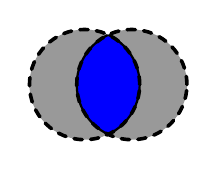
\begin{tikzpicture}[line width=1.3pt, line cap=round, line join=round, >=Stealth, x=1mm,y=1mm]
  \fill[gray!80] (-3,0) circle (7);
  \fill[gray!80] (3,0) circle (7);
  \begin{scope}
    \clip (-3,0) circle (7);
    \fill[blue] (3,0) circle (7);
  \end{scope}
  \draw[dashed] (-3,0) circle (7);
  \draw[dashed] (3,0) circle (7);
  \begin{scope}
    \clip (-3,0) circle (7);
    \draw[thick] (3,0) circle (7);
  \end{scope}
  \begin{scope}
    \clip (3,0) circle (7);
    \draw[thick] (-3,0) circle (7);
  \end{scope}
\end{tikzpicture}
\end{document}
